\section{MatrixRTC}\label{matrixRTC}

Lorem

\subsection{Využití Matrix primitivů}

Lorem

\subsection{Struktura Matrix eventů}

Takto vypadá \mintinline{typescript}{m.call} state event:

\begin{minted}{json}
{
	"type": "m.call",
	"state_key": "cvsiu2893",
	"content": {
		"m.intent": "m.room",
		"m.type": "m.voice",
		"m.name": "Voice room"
	}
}
\end{minted}

\subsection{Client SDKs}

Lorem

\subsection{Foci}

Lorem

\begin{figure}[h]
	\centering
	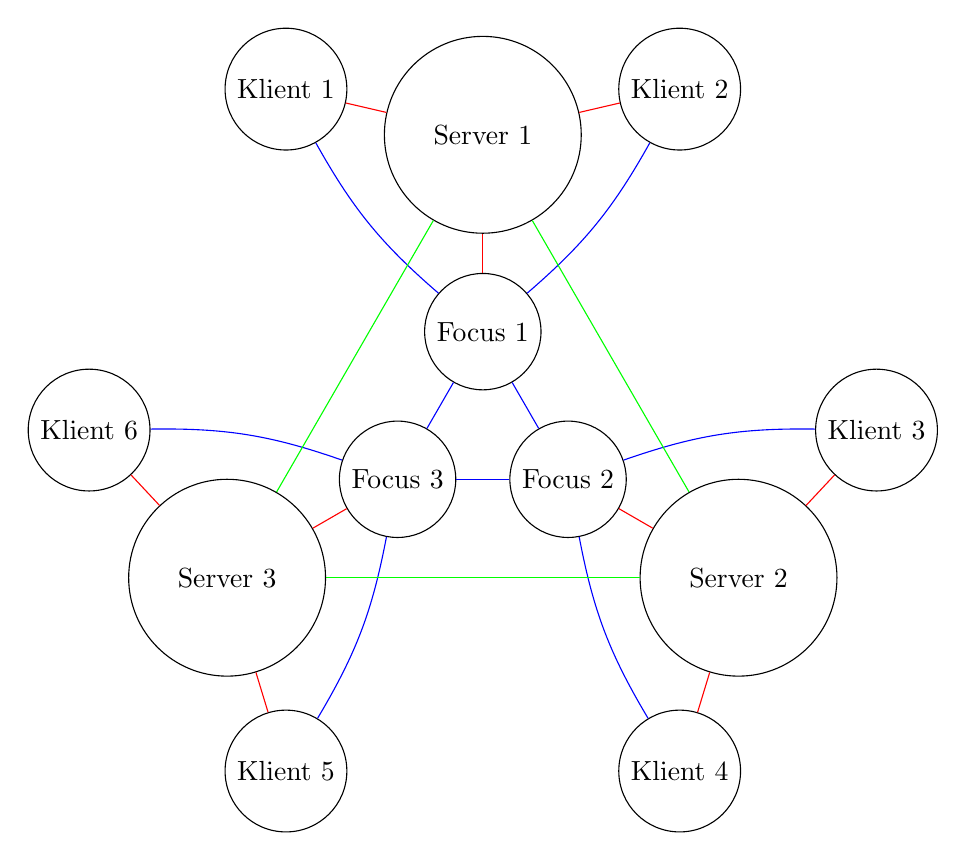
\begin{tikzpicture}[every node/.style={draw,circle}]
		\foreach \i in {1,...,3} {
				\node (focus\i) at ({90-360/3*(\i-1)}:1.25) {Focus \i};
				\node[minimum size=2.5cm] (server\i) at ({90-360/3*(\i-1)}:3.75)
				{Server \i};

				\draw[red] (server\i) -- (focus\i);
			}

		\foreach \i in {1,...,3} {
				\node (client\i) at ({120-360/3*(\i-1)}:5) {Klient {\the\numexpr((\i-1)*2+1)}};

				\draw[red] (server\i) -- (client\i);
				\draw[blue] (focus\i) edge[bend left=10] (client\i);
			}
		\foreach \i in {1,...,3} {
				\node (client{3+\i}) at ({60-360/3*(\i-1)}:5) {Klient {\the\numexpr((\i-1)*2+2)}};

				\draw[red] (server\i) -- (client{3+\i});
				\draw[blue] (focus\i) edge[bend right=10] (client{3+\i});
			}

		\foreach \i in {1,...,2} {
				\foreach \j in {\the\numexpr\i+1,...,3} {
						\draw[green] (server\i) -- (server\j);
						\draw[blue] (focus\i) -- (focus\j);
					}
			}
	\end{tikzpicture}
	\caption{Federace Matrix foci}
	\label{federatedFoci}
\end{figure}
